\chapter{Teoretski uvod}
\label{chap:teoretski-uvod}

\section{Homologija proteina}
\label{sec:homologija}

Homologija u biološkom smislu predstavlja slične osobine među vrstama na
različitim razinama organizacije života, poput organa, tkiva, stanice ili
molekule. Homologne osobine uočene među jedinkama različitih vrsta obično
upućuju na zajedničke pretke tih vrsta u evoluciji. Međutim, u molekularnoj
biologiji termin homolog se često koristi i za naznačavanje sličnosti. bez
obzira na genetsko srodstvo.\cite{bioinfo1}

\begin{figure}[h!]
\centering
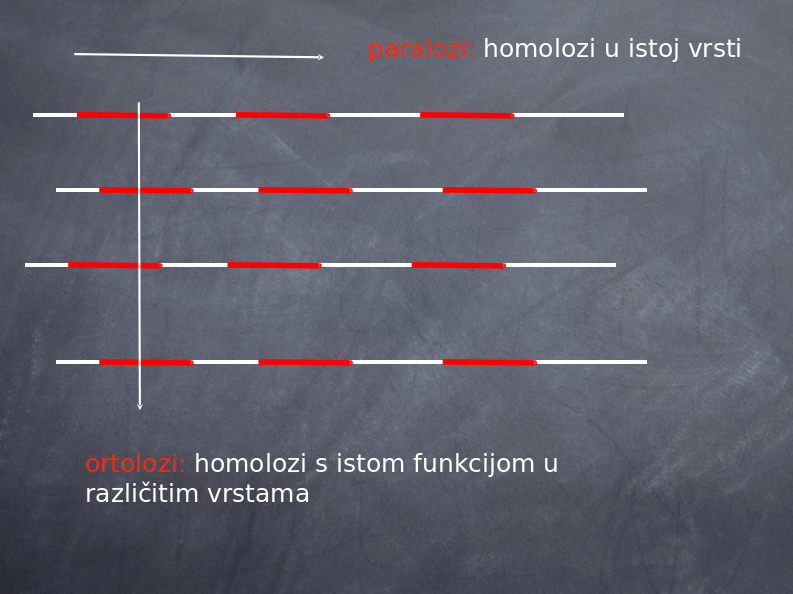
\includegraphics[width=4.5in]{figures/ortho-para.png}
\caption{Vizualni prikaz ortolognih i paralognih gena na genetskim lancima
raznih vrsta}
\label{fig:para-ortho}
\end{figure}

Za homologne sekvence proteina kažemo da su ortologne kad su direktni
potomci neke sekvence u zajedničkom pretku, bez da su prošle duplikaciju
gena. Drugim riječima, ortologne sekvence se mogu naći u jedinkama
različitih vrsta, a obavljaju istu ili sličnu funkciju u svim tim vrstama.
Paralogne sekvence su homologne sekvence koje su nastale od dvije različite
kopije nekog gena koji je prošao kroz proces duplikacije gena u nekom
zajedničkom evolucijskom pretku. Paralozi se mogu naći u jedinkama jedne ili
više vrsta te ne obavljaju nužno identične funkcije. Slika \ref{fig:para-ortho}
predočuje razliku paraloga i ortologa.


\section{Uloge proteina}
\label{sec:uloge}

Proteini, ili neki njihovi dijelovi koji imaju ključne uloge u stanicama su
često toliko bitni da kroz generacije vrsta vrlo malo mutiraju. Takva pojava se
naziva evolucijski pritisak. Znajući koji su dijelovi proteina dobro očuvani,
odnosno pod evolucijskim pritiskom, detaljnijim promatranjima i eksperimentima
se može utvrditi uloga i značenje tog očuvanog dijela proteina.

Postupak kojim se ovo postiže je sljedeći. Sekvence promatranih proteina se
poravnaju i pronađu se pozicije na kojima su reziduumi aminokiselina jednaki,
ili približno jednaki među svim sekvencama. Međutim, donošenje odluka o
srodnosti na ovakav način je statističke naravi. Drugim riječima, nitko ne može
garantirati da su dvije sekvence slične samo zato što imaju zajedničkog pretka.
Ipak, što je veća sličnost, to je veća vjerojatnost da sekvence doista jesu
srodne jer vjerojatnost slučajnog nastanka sličnih sekvenci geometrijski opada s
porastom podudarnosti. Zato je potrebno imati velik skup uzoraka potpuno
sekvenciranih genoma kako bi se definitivno moglo zaključiti jesu li geni, to
jest njihovi produkti --- proteini, srodni.


\section{Problemi i pretpostavke}
\label{sec:pp}

Pitanje koje se prirodno sljedeće postavlja jest kako zaključiti imaju li dva
proteina istu ulogu. Prva pretpostavka koja se ovdje donosi jest da ortolozi
imaju jednake uloge. Ova je činjenica u glavnom točna i u odsutnosti
eksperimentalne verifikacije ne može se biti precizniji. Dakle, određeni protein
od interesa bi u glavnom željeli usporediti sa skupom njoegovih ortologa.

Sada smo došli do problema prikupljanja skupa ortologa za dani protein. Kako bi
se pristupilo ovom problemu, donosi se druga pretpostavka: ortolozi se mogu
pronaći pretragom \emph{uzajamno najboljeg pogotka} potpunih skupova paraloga iz
dvije vrste.

Jedini način korištenja dva poptuna skupa paraloga jest da pretražujemo cijele
genome. Međutim, trenutno postoji jako malo cjelokupnih sekvencioniranih genoma,
a i oni koji su poznati su pretežito uzimani iz kralježnjaka. Uz to,
sekvencioniranje genoma i detekcija gena su skloni pogreškama. Alternativni
pristup, na kojem počiva ideja za Orthobalancera, jest potražiti informacije u
bazama podataka gdje se mogu naći individualne proteinske sekvence bez obzira na
činjenicu je li ostatak genoma vrste koja sadrži protein poznat. Nakon
skupljanja sekvenci sličnih polaznom proteinu, postavljaju se dva pitanja:

\begin{enumerate}

    \item Koje sekvence su ortologne polaznom proteinu?

    \item Koje taksonomske grane naš uzorak pokriva?

\end{enumerate}
Prvom pitanju pristupamo tako da prikupimo slične proteine danom proteinu i
uzimamo najsličniji protein iz pojedine vrste kao ortolog. Na drugo pitanje
možemo odgovoriti stavljajući vrste, koje se pojavljuju u prikupljenim
ortolozima, automatski na taksonomsko stablo živog svijeta.

Treća pretpostavka jest da taksonomsko stablo aproksimira evolucijsko stablo.
Koristeći ovu pretpostavku i obilježene vrste dvaju skupova ortologa na
taksonomskom stablu te penjući se po stablu sve dok se označene grane ne spoje
za oba skupa, dobiva se uvid u brzinu mutacije, odnosno razinu evolucijskog
pritiska pojedinih dijelova proteina iz tih dvaju skupova.

Moguća zamka na koju se nailazi ovim pristupom jest da jedan od skupova ortologa
sadrži proteine iz vrsta koje se na taksonomskom stablu nalaze na potpuno
izdvojenoj grani koja ne sadrži vrste iz drugog skupa. Ovime bi se dobila kriva
procjena velike brzine mutacije, pogotovo u odnosu na uparene vrste na ostatku
stabla. Ovome problemu može se pristupiti na način da se odaberu čvorovi u
stablu --- zamjenski čvorovi --- ispod kojih se za svaki skup traže
'reprezentativne vrste, pokušavajući se balansirati što bliže vrstama. U
ostatku taksonomskog stabla se prihvaćaju samo jedan-na-jedan pogodci vrsta među
skupovima, ako postoje. Neizbalansirane grane se na taj način izbacuju iz
analize, ostavljajući skupove vrsta koji su divergirali jednako daleko u
prošlosti.


